\chapter{Conception}

\section{Introduction}
Après avoir analysé les besoins et identifié les acteurs, ce chapitre présente la conception détaillée de l’application \textbf{Tarteel Maghreb}. 
Il décrit l’architecture générale du système, la structure physique, ainsi que les vues dynamique et navigation à travers des diagrammes UML. 
L’objectif est de garantir une compréhension claire de l’organisation et du fonctionnement de l’application avant son développement.

\section{Architecture générale}
L’application repose sur une architecture client-serveur simple et efficace, composée de trois principaux composants : 
\begin{itemize}
    \item \textbf{Client mobile} : l’application React Native installée sur le smartphone de l’utilisateur. Elle permet l’enregistrement audio, la lecture du Coran, l’affichage des résultats et l’interaction avec le serveur.
    \item \textbf{Serveur Node.js} : gère les requêtes provenant du client, fournit les données nécessaires pour l’application et communique avec le serveur IA pour l’analyse des récitations.
    \item \textbf{Serveur IA (FastAPI + Whisper)} : analyse les fichiers audio reçus du client via le serveur Node.js et renvoie un retour pédagogique sur la récitation.
\end{itemize}


\section{Diagramme de contexte}
Le diagramme de contexte montre les interactions principales entre les acteurs et le système \textbf{Tarteel Maghreb}. Les échanges concernent principalement : l’envoi de fichiers audio, la réception des résultats de récitation et l’accès aux fonctionnalités de lecture du Coran.

\begin{figure}[H]
\centering
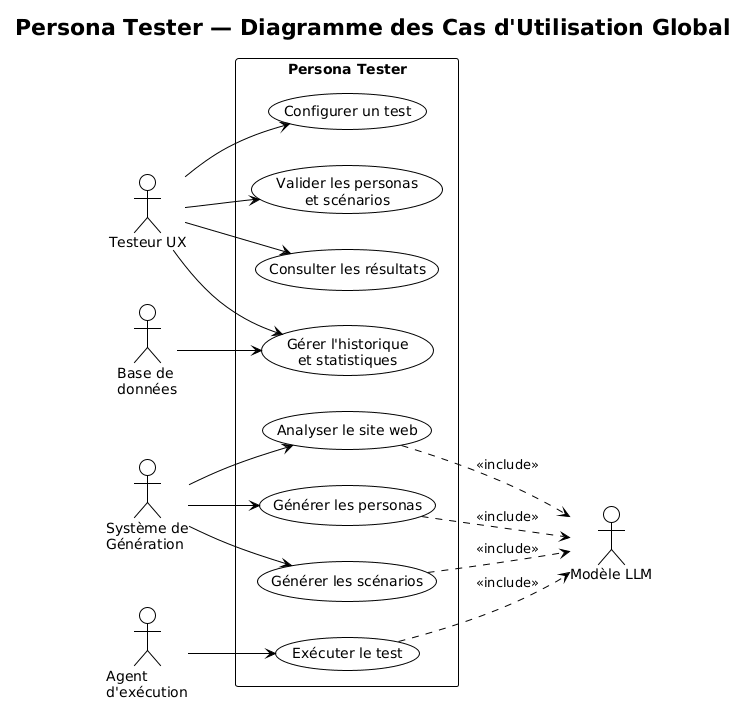
\includegraphics[height=70mm]{images/diagramme-usecase.png}
\caption{Diagramme de contexte simplifié}
\end{figure}

\section{Architecture physique}
L’architecture physique décrit la répartition du système sur les différents composants matériels et serveurs :  

\begin{itemize}
    \item \textbf{Appareil mobile} : exécution de l’application client, enregistrement audio, lecture des sourates et affichage des résultats.
    \item \textbf{Serveur Node.js} : héberge l’API REST qui reçoit les requêtes du client et transmet les fichiers audio au serveur IA.
    \item \textbf{Serveur IA (FastAPI + Whisper)} : analyse les fichiers audio et renvoie le feedback au serveur Node.js pour qu’il soit affiché sur le client mobile.
    \item \textbf{Stockage cloud } : sauvegarde des fichiers audio ou résultats pour permettre l’accès ultérieur depuis différents appareils.
\end{itemize}

\begin{figure}[H]
\centering
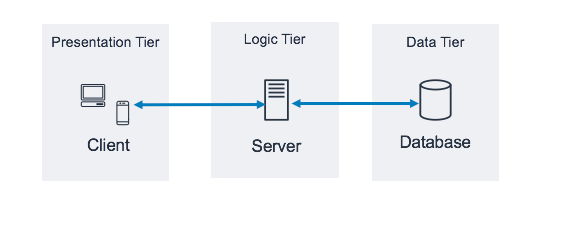
\includegraphics[height=70mm]{images/Architecture-physique-tiers.png}
\caption{Architecture physique du système client-serveur avec serveur IA}
\end{figure}

\section{Vue dynamique}
La vue dynamique décrit le flux des opérations lors de la récitation : de l’enregistrement audio par l’utilisateur, à l’envoi au serveur Node.js, à l’analyse par le serveur IA et au retour du feedback.

\begin{figure}[H]
\centering
\includegraphics[height=90mm]{images/sequence.png}
\caption{Diagramme de séquence pour la gestion des récitations}
\end{figure}

\section{Navigation et interface utilisateur}
L’interface mobile a été conçue pour faciliter la navigation entre les principales sections : 
\begin{itemize}
    \item Bibliothèque des sourates ;
    \item Lecteur audio intelligent ;
    \item Mode exercice avec feedback en temps réel.
\end{itemize}

\begin{figure}[H]
\centering
\includegraphics[height=70mm]{images/Structure de navigation de l'application.png}
\caption{Diagramme de navigation et interface utilisateur}
\end{figure}

\section{Conclusion}
Ce chapitre a présenté la conception détaillée de l’application \textbf{Tarteel Maghreb} avec une architecture client-serveur simplifiée.  
La répartition entre client mobile, serveur Node.js et serveur IA assure modularité et clarté.  
La vue dynamique et la navigation permettent de comprendre le flux des interactions et l’expérience utilisateur, garantissant que toutes les fonctionnalités identifiées dans le chapitre des besoins seront correctement implémentées.
